\section{Results}
The results presented for each scenario include the energy produced, reactor 
deployment schedule, enriched
uranium mass, \gls{HALEU} mass, and \gls{SWU} capacity required as a function of time. 

\subsection{Scenario 1}
The amount of energy supplied by the \glspl{LWR} and the number of \glspl{LWR}
deployed as a function of time is shown in Figure \ref{fig:energy_rx_1}. 
\glspl{LWR} are first deployed in August of 1967, and the last 
\gls{LWR} is decommissioned in June of 2016. The maximum number of 
\glspl{LWR} deployed at one time is 109. The energy produced by the 
\glspl{LWR} follows with the number of reactors deployed. The maximum energy 
produced by the \glspl{LWR} is 102.46 GWe-y, and they produce 91.82 GWe-y 
in 2025.

\begin{figure}
    \centering 
    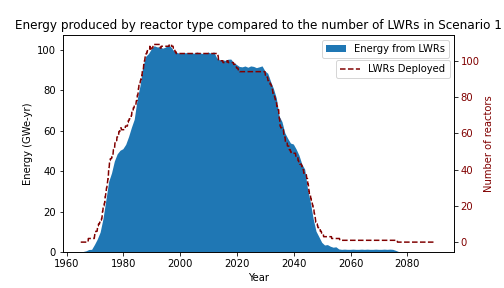
\includegraphics[scale=0.5]{figures/energy_scenario1.png}
    \caption{Energy supplied by \glspl{LWR} compared to the number of 
    \glspl{LWR} deployed in Scenario 1.}
    \label{fig:energy_rx_1}
\end{figure}

The mass of enriched uranium sent to the \glspl{LWR} at each 
time step is shown in Figure \ref{fig:fuel_1}. The \glspl{LWR} are 
defined to have an 18 month cycle length, with a third of the uranium 
mass replaced at each refueling outage. However, when a new reactor 
is deployed it is deployed with an entire core of uranium which leads 
to the large increases in the mass of uranium sent to the reactors, such 
as in 1983 and 2016. An average of 96.2 MTU/month and a maximum of 513.7 MTU 
is sent to the \glspl{LWR}. Prior to 2025, the average mass
of enriched uranium sent to the \glspl{LWR} is 157.6 MTU/month. 

\begin{figure}
    \centering 
    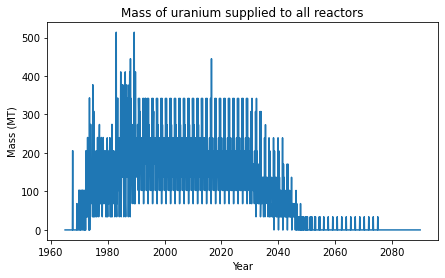
\includegraphics[scale=0.5]{figures/fuelsupply_scenarios_1.png}
    \caption{Mass of enriched uranium sent to reactors in Scenario 1.}
    \label{fig:fuel_1}
\end{figure}

Finally, the \gls{SWU} capacity to produce fuel for the scenario is shown in 
Figure \ref{fig:swu_1}. The \gls{SWU} capacity required as a function of 
time follows the mass of uranium sent to the reactors, since the \gls{SWU}
is calculated based on those transactions. An average of 0.74$\times 10^6$
kg-\gls{SWU}/month and a maximum of 3.95$\times 10^6$ kg-\gls{SWU} is 
required for this scenario. Prior to 2025, an average of 1.21$\times 10^6$ 
kg-\gls{SWU}/month is required to enrich the uranium sent to the \glspl{LWR}.

\begin{figure}
    \centering
    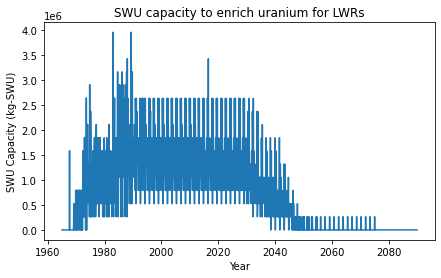
\includegraphics[scale=0.5]{figures/totalswu_scenarios_1.png}
    \caption{Total \gls{SWU} capacity required to produce fuel sent to the 
    reactors at each time step in Scenario 1.}
    \label{fig:swu_1}
\end{figure}

The deployment schedule of the \glspl{LWR} in this scenario is 
applied to each of the other scenarios, and therefore the material 
requirements of each of the following scenarios is the same as those 
of this scenario prior to 2025. 

\subsection{Scenario 2}
The energy produced by each type of reactor, the transition energy demand, 
and the deployment schedule of the \glspl{MMR} for Scenario 2 are shown in 
Figure \ref{fig:energy_rx_2}. The first \glspl{MMR} are deployed in 
October 2031, and the 
maximum number deployed at one time is 
9,182. The deployment of \glspl{MMR} in 2031 contributes to the inability to 
meet the energy demand of the scenario because the energy produced by 
\glspl{LWR} decreases to 89.35 GWe-y in 2030, before the \glspl{MMR} are 
deployed. Therefore, the reactors are deployed in a reactionary fashion to 
past energy production, as opposed to in response to forecasted energy 
production.

Once the transition begins in 2025, there are 
clearly some time periods in which the energy demand of the scenario is 
not met. The first of these is between 2030-2050, with a maximum deficit 
of 5.7855 GWe-y in 2032. Other periods in which the energy demand is not met 
correspond to the decommissioning of \glspl{MMR} at the end of their lifetime 
and the deployment of new reactors, such as from 2062-2069. 

\begin{figure}
    \centering 
    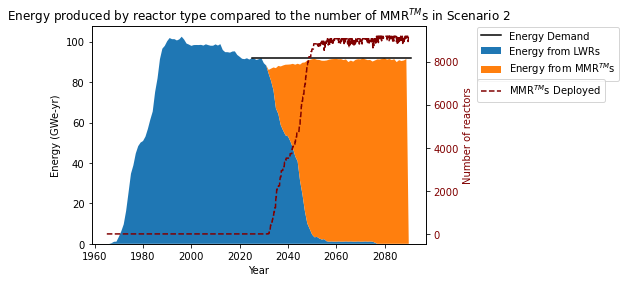
\includegraphics[scale=0.5]{figures/energy_scenario2.png}
    \caption{Energy supplied by each type of reactor compared to the number of 
    \glspl{MMR} deployed in Scenario 2.}
    \label{fig:energy_rx_2}
\end{figure}

Figure \ref{fig:fuel_2} shows the mass of enriched uranium sent to all 
reactors in the scenario and just to the \glspl{MMR}. The \glspl{MMR} 
do not require refueling during their lifetime, so uranium is only 
sent to these reactors when they are deployed. This causes the 
large, sudden increases in uranium sent to these reactors and the periods of 
no uranium sent to them. An average of 104.94 MTU/month and a maximum 
of 781.41 MTU is sent to all of the reactors in the scenario after 2025. 
This average is lower than the average mass of enriched uranium 
sent to the \glspl{LWR} in Scenario 1, but the maximum value is 267.71 MTU 
more than the maximum mass of enriched uranium sent to the \glspl{LWR} in 
Scenario 1. 

An average of 48.50 MTU/month and a maximum of 719.25 
MTU is sent to the \glspl{MMR} once they are deployed in 2031. The average 
mass of enriched uranium sent to the 
\glspl{MMR} is higher than the average mass of uranium sent to the \glspl{LWR}
prior to 2025. This is despite a much higher maximum and multiple peaks higher
than
average mass sent to the \glspl{LWR}. The lower average is explained by the 
multiple time periods in 
which no \gls{HALEU} is sent to the \glspl{MMR}.  

\begin{figure}
    \centering
    \begin{subfigure}{0.4\textwidth}
        \centering
        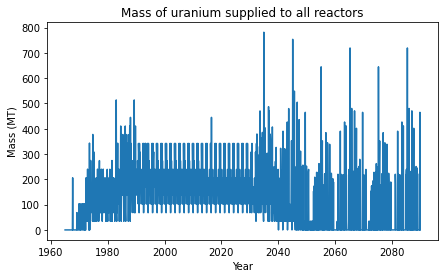
\includegraphics[scale=0.3]{figures/fuelsupply_scenarios_2.png}
        \caption{Mass of enriched uranium sent to all reactors.}
        \label{fig:totalfuel_2}
    \end{subfigure}
    \hspace{0.8cm}
    \begin{subfigure}{0.4\textwidth}
        \centering
        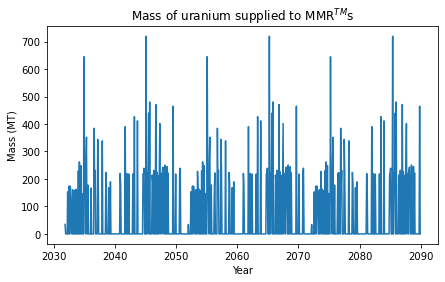
\includegraphics[scale=0.3]{figures/advancedRX_fuelsupply_scenarios_2.png}
        \caption{Mass of enriched uranium sent to \glspl{MMR}.}
        \label{fig:haleu_2}
    \end{subfigure}
    \caption{Uranium mass sent to reactors in Scenario 2.}
    \label{fig:fuel_2}
\end{figure}

Figure \ref{fig:swu_2} shows the \gls{SWU} capacity needed to 
enrich uranium for all reactors in the scenario, and to enrich uranium for 
just the \glspl{MMR}. There is a large difference in the \gls{SWU} 
capacity needed to enrich uranium for \glspl{LWR} and \glspl{MMR}. This 
is because the \glspl{MMR} require a much larger mass and 
a higher enrchment level. An average of 1.37$\times 10^6$ kg-\gls{SWU}/month
and a maximum of 20.3$\times 10^6$ kg-\gls{SWU}
is needed to enrich the uranium sent to \glspl{MMR}. These values are both 
higher than the 
average and maximum \gls{SWU} capacity needed to enrich fuel for the 
\glspl{LWR} in Scenario 1. 


\begin{figure}
    \centering
    \begin{subfigure}{0.4\textwidth}
        \centering
        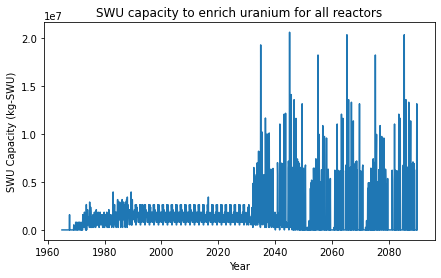
\includegraphics[scale=0.3]{figures/totalswu_scenarios_2.png}
        \caption{Total \gls{SWU} required to enrich uranium sent to all reactors at each time step.}
        \label{fig:totalswu_2}
    \end{subfigure}
    \hspace{0.8cm}
    \begin{subfigure}{0.4\textwidth}
        \centering
        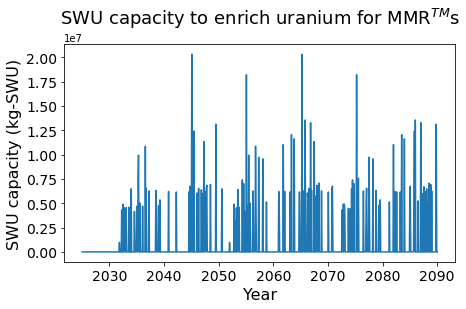
\includegraphics[scale=0.3]{figures/haleuSWU_scenarios_2.png}
        \caption{\gls{SWU} required to enrich uranium sent to \glspl{MMR} at each time step.}
        \label{fig:haleuswu_2}
    \end{subfigure}
    \caption{\gls{SWU} required to enrich natural uranium in Scenario 2.}
    \label{fig:swu_2}
\end{figure}

\subsection{Scenario 3}
Figure \ref{fig:energy_rx_3} shows the number of Xe-100 reactors deployed, 
the energy produced by each reactor type, and the energy demand of Scenario 3. 
Xe-100 reactors are deployed in October 2031, which is the same as when 
\glspl{MMR}
are deployed in Scenario 2. A maximum of 1225 Xe-100 reactors are deployed.

The same deficit between the energy produced and demand between 
2030-2050 that was observed in Scenario 2 is present in the energy produced 
in this scenario. However, there are no significant 
differences (more than 1 GWe-y for this work) between the energy 
produced and demand of the scenario 
after 2050 because the Xe-100 reactors have a longer lifetime, and there are 
no decreases in energy due to decommissioning of reactors. After 2050, the 
maximum difference between the energy produced and demand is 0.057 GWe-y. 

\begin{figure}
    \centering 
    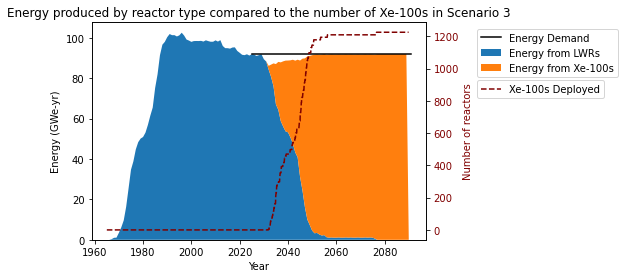
\includegraphics[scale=0.5]{figures/energy_scenario3.png}
    \caption{Energy supplied by each type of reactor compared to the number of 
    Xe-100s deployed in Scenario 3.}
    \label{fig:energy_rx_3}
\end{figure}

Figure \ref{fig:fuel_3} shows the mass of enriched uranium sent to all reactors,
and just to the Xe-100 reactors. The Xe-100 reactors 
require significantly less fuel than what is sent to the \glspl{LWR}, 
despite there being more Xe-100 reactors than \glspl{LWR}. Uranium 
is sent to the Xe-100 reactors every six months in the simulations, 
while it is sent to the \glspl{LWR} every 18 months. An average of 
74.98 MTU/month and a maximum of 342.58 MTU is sent to all of the reactors 
in this scenario starting in 2025. Both values are considerably
lower than in Scenario 1.

An average of 23.81 
MTU/month and a maximum of 105.67 MTU is sent to the Xe-100 reactors in 
this scenario. Each of these numbers are considerably lower than the 
average and maximum masses of enriched uranium  
in Scenario 1, and the \gls{HALEU} mass sent to the \glspl{MMR} in 
Scenario 2. 

\begin{figure}
    \centering
    \begin{subfigure}{0.4\textwidth}
        \centering
        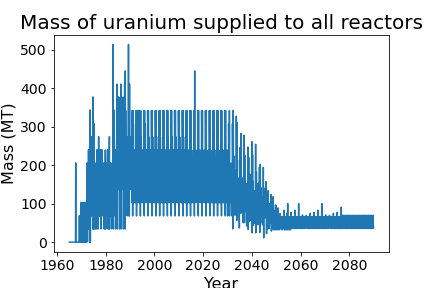
\includegraphics[scale=0.3]{figures/fuelsupply_scenarios_3.png}
        \caption{Mass of enriched uranium sent to all reactors.}
        \label{fig:totalfuel_3}
    \end{subfigure}
    \hspace{0.8cm}
    \begin{subfigure}{0.4\textwidth}
        \centering
        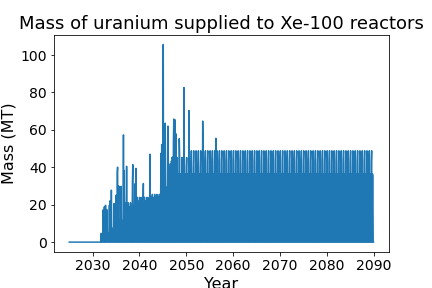
\includegraphics[scale=0.3]{figures/advancedRX_fuelsupply_scenarios_3.png}
        \caption{Mass of enriched uranium sent to Xe-100s.}
        \label{fig:haleu_3}
    \end{subfigure}
    \caption{Uranium mass sent to reactors in Scenario 3.}
    \label{fig:fuel_3}
\end{figure}

Figure \ref{fig:swu_3} shows the \gls{SWU} capacity needed to enrich 
uranium for all of the reactors in the scenario, and for the uranium sent 
to just the Xe-100 reactors. There is no substantial change in the 
\gls{SWU} capacity needed to enrich uranium for the \glspl{LWR} in 
Scenario 1 and for the Xe-100 
reactors in this scenario, despite the higher enrichment level of uranium 
sent to the Xe-100 reactors. This is because the Xe-100 reactors are sent 
a lower average mass of enriched uranium at each time step. Enriching uranium 
for the Xe-100 reactors requires an average of 
0.82$\times 10^6$ kg-\gls{SWU}/timestep and a maximum of 3.64$\times 10^6$
kg-\gls{SWU}. These values are comparable to what is required to enrich 
uranium in Scenario 1. 

\begin{figure}
    \centering
    \begin{subfigure}{0.4\textwidth}
        \centering
        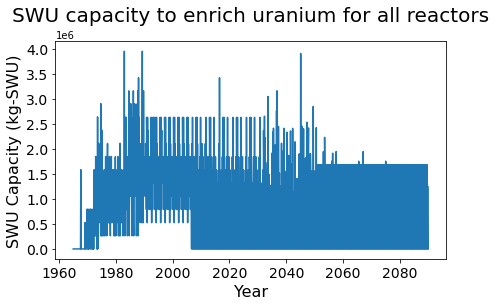
\includegraphics[scale=0.3]{figures/totalswu_scenarios_3.png}
        \caption{\gls{SWU} required to enrich uranium sent to all reactors.}
        \label{fig:totalswu_3}
    \end{subfigure}
    \hspace{0.8cm}
    \begin{subfigure}{0.4\textwidth}
        \centering
        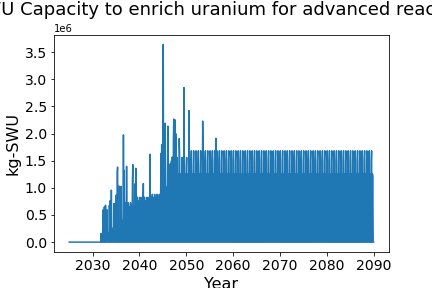
\includegraphics[scale=0.3]{figures/haleuSWU_scenarios_3.png}
        \caption{\gls{SWU} required to enrich uranium sent to Xe-100s.}
        \label{fig:haleuswu_3}
    \end{subfigure}
    \caption{\gls{SWU} required to enrich natural uranium in Scenario 3.}
    \label{fig:swu_3}
\end{figure}

\subsection{Scenario 4}
Figure \ref{fig:energy_rx_4} shows the number of \glspl{MMR} deployed, 
energy produced by each type of reactor, and the energy demand of the 
scenario. \glspl{MMR} are deployed in January 2030, and the maximum 
number of \glspl{MMR} is 17,496. 

There is a small deficit between the energy produced and  
demand from 2026-2046, with a maximum difference of 4.51 GWe-y in 2032.
There are no other times in which the energy demand is not met by a 
significant amount (more than 1 GWe-y), including when the \glspl{MMR} are 
decommissioned. After 2047 electricity is generally produced in surplus, 
up to 1.64 GWe-y. 

\begin{figure}
    \centering 
    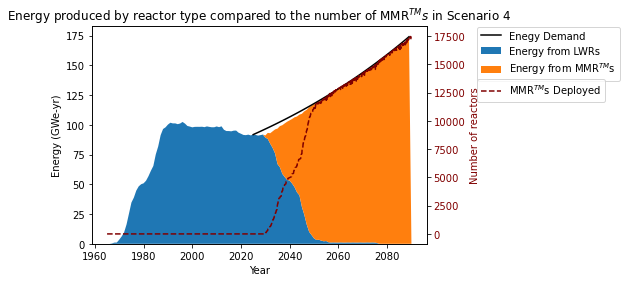
\includegraphics[scale=0.5]{figures/energy_scenario4.png}
    \caption{Energy supplied by each type of reactor compared to the number of 
    \glspl{MMR} deployed in Scenario 4.}
    \label{fig:energy_rx_4}
\end{figure}

Figure \ref{fig:fuel_4} shows the mass of enriched uranium sent to all the 
reactors in the scenario, and to just the \glspl{MMR} 
in the scenario. An average of 144.36 MTU/month and a maximum of 796.71 MTU
is sent to all the reactors starting in 2025 in this scenario. An average of 
75.62 MTU/month and a maximum of 755.60 MTU is sent to just the \glspl{MMR}
in the scenario once they are deployed. Unsurprisingly, the mass of \gls{HALEU}
required by the \glspl{MMR} in this scenario is higher than  
in Scenario 2 due to the higher energy 
demand and the higher number of \glspl{MMR} deployed in this scenario. The 
average mass of \gls{HALEU} sent to the \glspl{MMR} in this scenario is 
slightly lower than the average mass sent to the \glspl{LWR} in Scenario 1 
due to the multiple time steps in which no uranium is sent to the \glspl{MMR}.

\begin{figure}
    \centering
    \begin{subfigure}{0.4\textwidth}
        \centering
        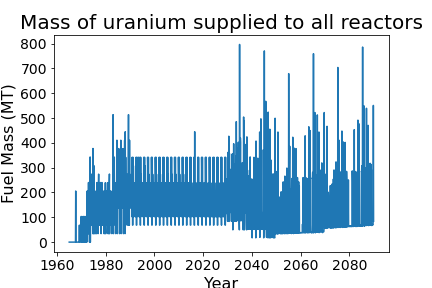
\includegraphics[scale=0.3]{figures/fuelsupply_scenarios_4.png}
        \caption{Mass of enriched uranium sent to all reactors.}
        \label{fig:totalfuel_4}
    \end{subfigure}
    \hspace{0.8cm}
    \begin{subfigure}{0.4\textwidth}
        \centering
        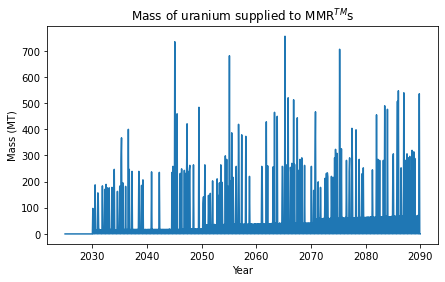
\includegraphics[scale=0.3]{figures/advancedRX_fuelsupply_scenarios_4.png}
        \caption{Mass of enriched uranium sent to \glspl{MMR}.}
        \label{fig:haleu_4}
    \end{subfigure}
    \caption{Uranium mass sent to reactors in Scenario 4.}
    \label{fig:fuel_4}
\end{figure}

Figure \ref{fig:swu_4} shows the \gls{SWU} capacity required to 
enrich uranium for all the reactors in the scenario, and 
only for the \glspl{MMR}. The \gls{SWU} capacity required to enrich uranium 
for the \glspl{MMR} is much higher than the capacity needed to 
enrich uranium for the \glspl{LWR} in the scenario because
the \glspl{MMR} require a much higher mass of enriched uranium 
and a higher enrichment level. An average of 2.19$\times 10^6$ 
kg-\gls{SWU}/month and a maximum of 21.5$\times 10^6$ kg-\gls{SWU}
is required to enrich the uranium that is sent to \glspl{MMR}. These values 
are higher than the \gls{SWU} 
capacity required to enrich uranium for the \glspl{MMR} in 
Scenario 2, but slightly higher than the average \gls{SWU} capacity 
required to enrich uranium for the \glspl{LWR} in Scenario 1. 

\begin{figure}
    \centering
    \begin{subfigure}{0.4\textwidth}
        \centering
        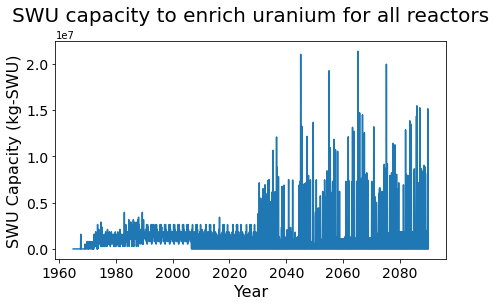
\includegraphics[scale=0.3]{figures/totalswu_scenarios_4.png}
        \caption{\gls{SWU} required to enrich uranium sent to all reactors.}
        \label{fig:totalswu_4}
    \end{subfigure}
    \hspace{0.8cm}
    \begin{subfigure}{0.4\textwidth}
        \centering
        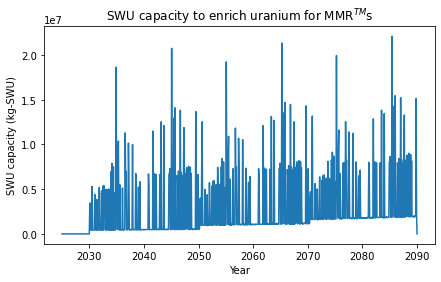
\includegraphics[scale=0.3]{figures/haleuSWU_scenarios_4.png}
        \caption{\gls{SWU} required to enrich uranium sent to \glspl{MMR}.}
        \label{fig:haleuswu_4}
    \end{subfigure}
    \caption{\gls{SWU} required to enrich natural uranium in Scenario 4.}
    \label{fig:swu_4}
\end{figure}


\subsection{Scenario 5}
Figure \ref{fig:energy_rx_5} shows the number of Xe-100 reactors, the 
energy produced by each type of reactor, and the energy demand of the 
scenario. The Xe-100 reactors are deployed in January 2030, the 
same as when 
\glspl{MMR} are deployed in Scenario 4. The maximum number of Xe-100 
reactors deployed in the scenario is 2339. 

There is a small deficit in the energy produced and demand from 
2026-2046, the same as what was observed in Scenario 4. After this 
initial difference, there are no further significant (more than 
1 GWe-y) differences between 
the energy produced and demand. For most years after 2046 there 
is a surplus of energy, up to 1.64 GWe-y. 

\begin{figure}
    \centering 
    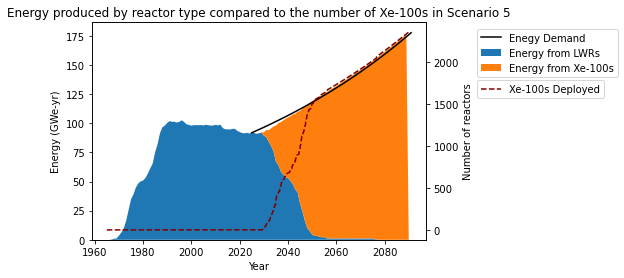
\includegraphics[scale=0.5]{figures/energy_scenario5.png}
    \caption{Energy supplied by each type of reactor compared to the number of 
    Xe-100s deployed in Scenario 5.}
    \label{fig:energy_rx_5}
\end{figure}

Figure \ref{fig:fuel_5} shows the mass of enriched uranium sent the all  
the reactors in the scenario and the \gls{HALEU} mass sent just to the 
Xe-100 reactors. There is a clear increase in the mass of \gls{HALEU} sent 
to the Xe-100 reactors as time goes on, but this mass is still  
low compared to the mass of enriched uranium sent to the \glspl{LWR} in 
the scenario. An average of 95.46 MTU/month and a maximum of 347.28 MTU 
is sent to all of the reactors in this scenario after 2025. These 
values are both lower than the uranium mass sent to the 
\glspl{LWR} in Scenario 1. An average of 
38.11 MTU/month and a maximum of 117.98 MTU is sent to the Xe-100 reactors. 
These metrics are all much lower than what is observed 
for fueling the \glspl{MMR} in Scenario 4.


\begin{figure}
    \centering
    \begin{subfigure}{0.4\textwidth}
        \centering
        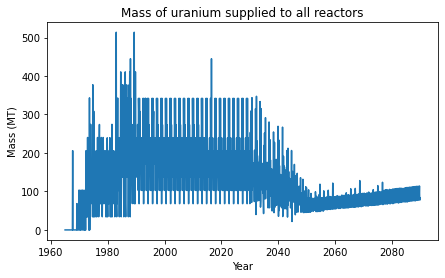
\includegraphics[scale=0.3]{figures/fuelsupply_scenarios_5.png}
        \caption{Mass of enriche uranium sent to all reactors.}
        \label{fig:totalfuel_5}
    \end{subfigure}
    \hspace{0.8cm}
    \begin{subfigure}{0.4\textwidth}
        \centering
        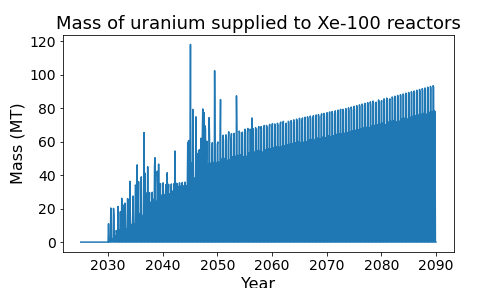
\includegraphics[scale=0.3]{figures/advancedRX_fuelsupply_scenarios_5.png}
        \caption{Mass of enriched uranium sent to Xe-100s.}
        \label{fig:haleu_5}
    \end{subfigure}
    \caption{Uranium mass sent to reactors in Scenario 5.}
    \label{fig:fuel_5}
\end{figure}

Finally, Figure \ref{fig:swu_5} shows the \gls{SWU} capacity required
to enrich the uranium sent to all of the reactors, and just the Xe-100
reactors. The \gls{SWU} capacity needed 
to enrich uranium for the Xe-100 reactors starts out at a similar 
amount as the \glspl{LWR}, but 
increases as the enrgy demand and the number of reactors increases. 
The \gls{SWU} capacity required to enrich uranium 
for the Xe-100 reactors becomes higher than the capacity 
required to enrich uranium for \glspl{LWR}, despite the Xe-100 
reactors requiring a lower mass of uranium because of the higher 
enrichment level of the fuel. An average of 1.36$\times 10^6$ 
kg-\gls{SWU}/month and a maximum of 
4.11$\times 10^6$ kg-\gls{SWU} is required to enrich the uranium sent 
to the Xe-100 reactors. The average \gls{SWU} capacity 
required to enrich uranium for the Xe-100 reactors is a little lower 
than the average capacity needed to enrich uranium for the \glspl{MMR}
in Scenario 4, but the maximum capacity required for this scenario is much 
lower than in Scenario 4. These values are slightly higher 
than what is observed to enrich uranium for the \glspl{LWR} in Scenario 1
prior to 2025.

\begin{figure}
    \centering
    \begin{subfigure}{0.4\textwidth}
        \centering
        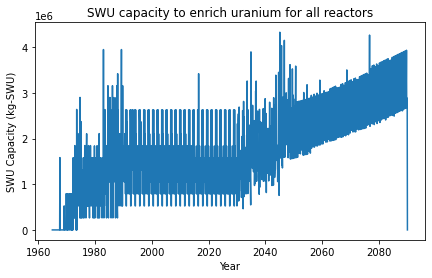
\includegraphics[scale=0.3]{figures/totalswu_scenarios_5.png}
        \caption{Total \gls{SWU} required to enrich uranium sent to all reactors at each time step.}
        \label{fig:totalswu_5}
    \end{subfigure}
    \hspace{0.8cm}
    \begin{subfigure}{0.4\textwidth}
        \centering
        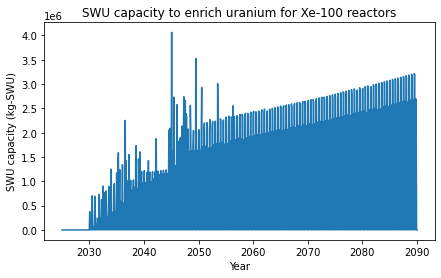
\includegraphics[scale=0.3]{figures/haleuSWU_scenarios_5.png}
        \caption{\gls{SWU} required to enrich uranium sent to Xe-100s at each time step.}
        \label{fig:haleuswu_5}
    \end{subfigure}
    \caption{\gls{SWU} required to enrich natural uranium in Scenario 5.}
    \label{fig:swu_5}
\end{figure}
